\documentclass[aspectratio=169]{beamer}
\usetheme{Madrid}
\usecolortheme{default}
\usepackage[utf8]{inputenc}
\usepackage[T5]{fontenc}
\usepackage{graphicx}
\usepackage{hyperref}
\usepackage{booktabs}
\usepackage{amsmath}
\usepackage{listings}
\usepackage{xcolor}

\setbeamertemplate{caption}[numbered]
\renewcommand{\figurename}{Hình}
\renewcommand{\thefigure}{19.\arabic{figure}}

\lstset{
    basicstyle=\ttfamily\scriptsize,
    breaklines=true,
    commentstyle=\color{green!60!black},
    keywordstyle=\color{blue},
    stringstyle=\color{orange},
    showstringspaces=false
}

\title[Chương 19: The Future of AI]{Học Sâu (Deep Learning) \\ \vspace{0.5cm} \Large Chương 19: Tương lai của Trí tuệ Nhân tạo (The Future of AI)}
\author{Đại học Đông Á}
\date{\today}

\begin{document}

\begin{frame}
    \titlepage
\end{frame}

\begin{frame}{Nội dung chương}
    \tableofcontents
\end{frame}

\section{1. Giới hạn của Deep Learning}

\begin{frame}{Bản chất thực sự của Deep Learning}
    \begin{columns}
        \column{0.5\textwidth}
        \begin{itemize}
            \item Mạng nơ-ron học sâu thực chất là những đường cong tham số khổng lồ (Parametric curves) được khớp (fit) với một lượng dữ liệu cực lớn.
            \item Mô hình không "suy nghĩ". Nó chỉ là một cơ sở dữ liệu \textbf{Nội suy tĩnh (Static Interpolative Database)}.
            \item Ở giai đoạn Inference, nó chỉ thực hiện truy xuất thông tin (Information retrieval) đã học.
        \end{itemize}
        
        \column{0.5\textwidth}
        \begin{figure}
            \centering
            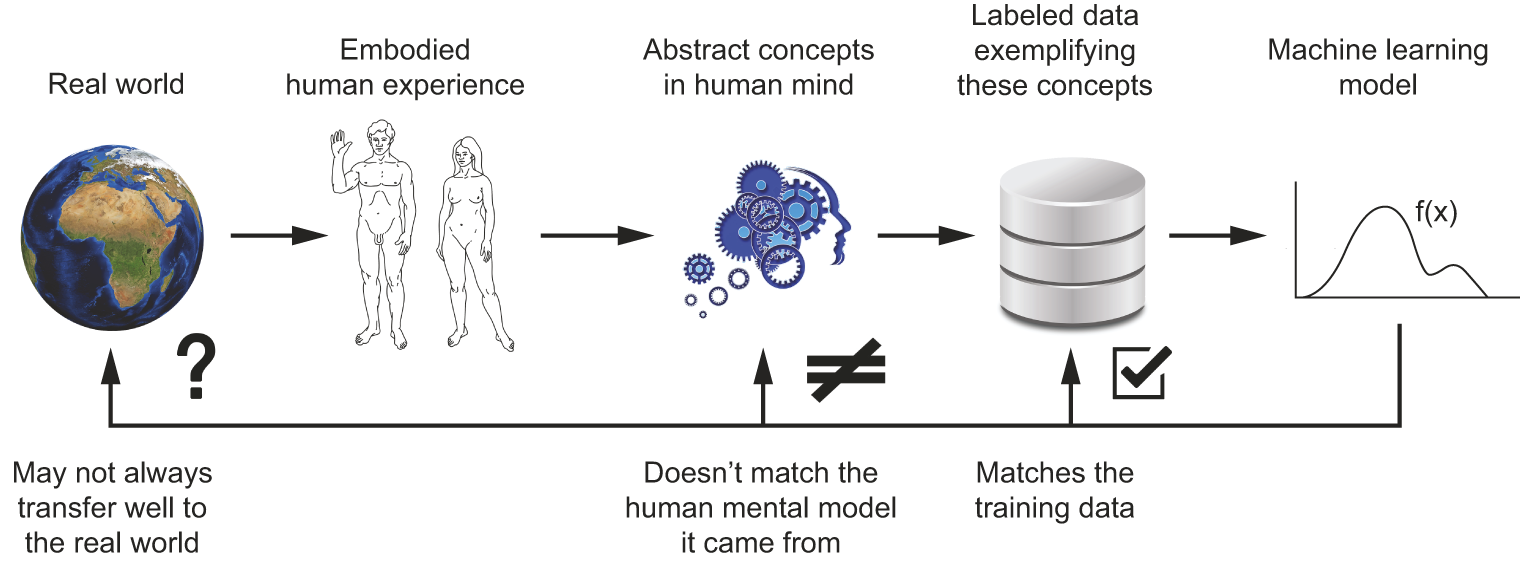
\includegraphics[width=\textwidth,height=0.6\textheight,keepaspectratio]{../../images/ch19/ml_model.02e47549.png}
            \caption{Mô hình ML như một cơ sở dữ liệu nội suy}
        \end{figure}
    \end{columns}
\end{frame}

\begin{frame}{Sự mù lòa trước cái mới (Novelty)}
    \begin{columns}
        \column{0.5\textwidth}
        \begin{itemize}
            \item Điểm yếu cốt tử của LLMs: Rất giỏi làm những thứ từng xuất hiện trên mạng, nhưng bất lực trước một bài toán \textbf{Mới hoàn toàn}, dù rất đơn giản.
            \item Hình bên là một bài kiểm tra logic rất dễ với con người. Nhưng do không có trong dữ liệu huấn luyện, LLM không thể giải quyết được.
            \item "Năng lực" của LLM phụ thuộc vào \textit{Sự quen thuộc} chứ không phải \textit{Trí thông minh}.
        \end{itemize}
        
        \column{0.5\textwidth}
        \begin{figure}
            \centering
            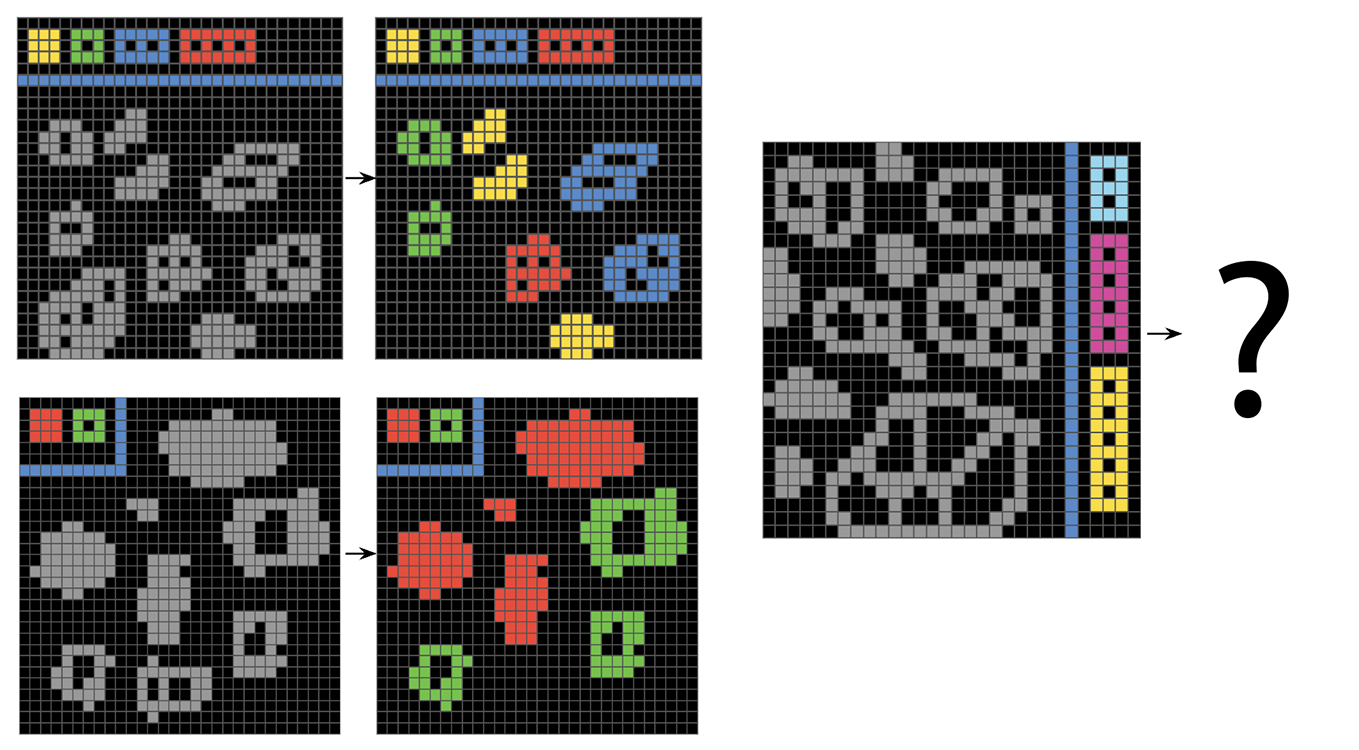
\includegraphics[width=\textwidth,height=0.6\textheight,keepaspectratio]{../../images/ch19/arc_example_2.7d4f0c33.png}
            \caption{Một câu đố logic đơn giản nhưng hoàn toàn mới}
        \end{figure}
    \end{columns}
\end{frame}

\begin{frame}{Vấn đề "Học vẹt" ở Large Language Models}
    \begin{columns}
        \column{0.5\textwidth}
        \begin{itemize}
            \item Thử nghiệm với bài toán Monty Hall (Biến thể).
            \item Nếu bạn đổi một số chi tiết trong bài toán gốc (Ví dụ: Cửa trong suốt), LLM vẫn nhả ra câu trả lời kinh điển mà nó đã học vẹt.
            \item Điều này chứng tỏ mô hình không mô phỏng lại hoàn cảnh vật lý, nó chỉ \textbf{dự đoán token tiếp theo} khớp với dữ liệu phân bố của nó.
        \end{itemize}
        
        \column{0.5\textwidth}
        \begin{figure}
            \centering
            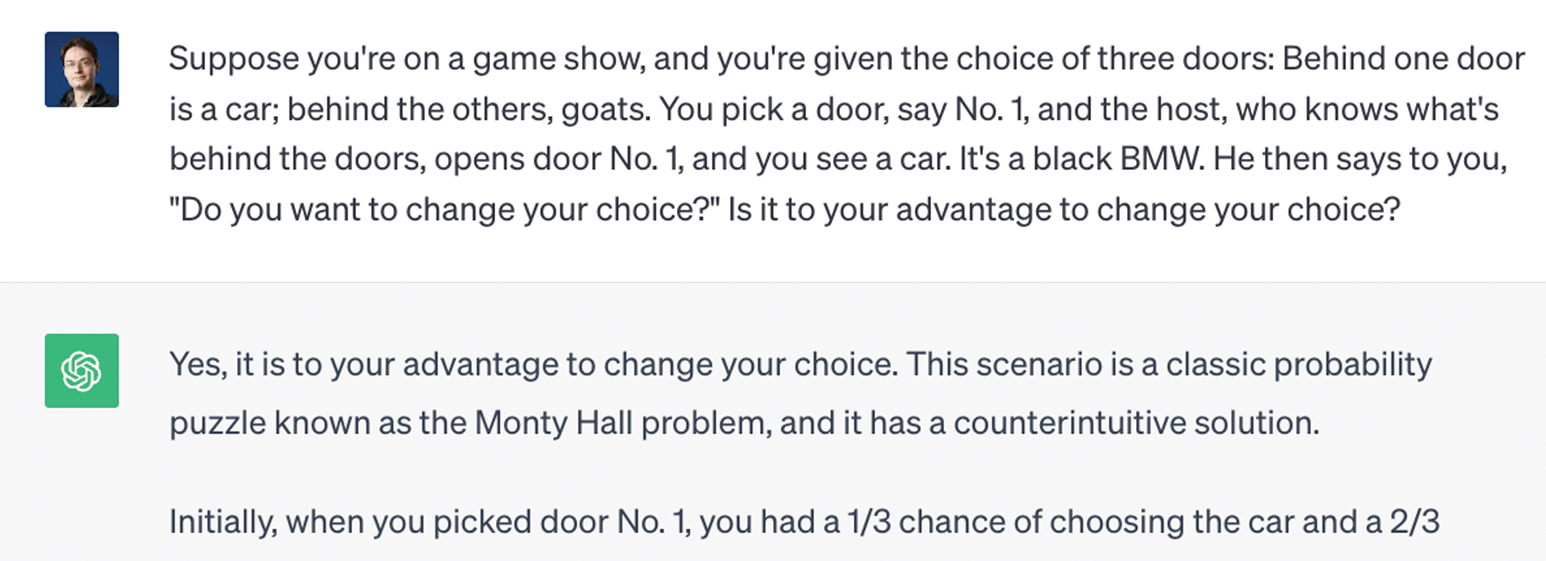
\includegraphics[width=\textwidth,height=0.6\textheight,keepaspectratio]{../../images/ch19/monty_hall.86dba4ca.png}
            \caption{Biến thể bài toán Monty Hall}
        \end{figure}
    \end{columns}
\end{frame}

\begin{frame}{Nhạy cảm với cách diễn đạt (Prompt Sensitivity)}
    \begin{itemize}
        \item Deep Learning cực kỳ nhạy cảm với cách trình bày đầu vào.
        \item LLM có thể trả lời đúng nếu cấu trúc câu hỏi giống dữ liệu huấn luyện, nhưng dễ dàng sai lệch khi thay đổi tên biến hoặc giá trị nhỏ.
        \item \textbf{Prompt Engineering} thực chất là tìm kiếm trong Không gian tiềm ẩn (Latent space) để trúng được mẫu dữ liệu tương tự mà mô hình đã học.
        \item Bản chất mô hình không thực sự hiểu câu lệnh, nó chỉ truy xuất theo độ tương đồng của văn bản đầu vào.
    \end{itemize}
\end{frame}

\begin{frame}{Gót chân Achilles: Mẫu đối kháng (Adversarial Examples)}
    \begin{columns}
        \column{0.5\textwidth}
        \begin{itemize}
            \item Deep Learning rất dễ bị đánh lừa bởi \textbf{Adversarial Examples}.
            \item Thêm một lớp nhiễu rất nhỏ (Mắt người không nhận ra) vào hình ảnh con heo, AI sẽ tự tin 99\% đây là một chiếc máy bay.
            \item Nguyên nhân: AI không học cấu trúc vật lý của con heo, nó học các phân bố điểm ảnh cục bộ.
        \end{itemize}
        
        \column{0.5\textwidth}
        \begin{figure}
            \centering
            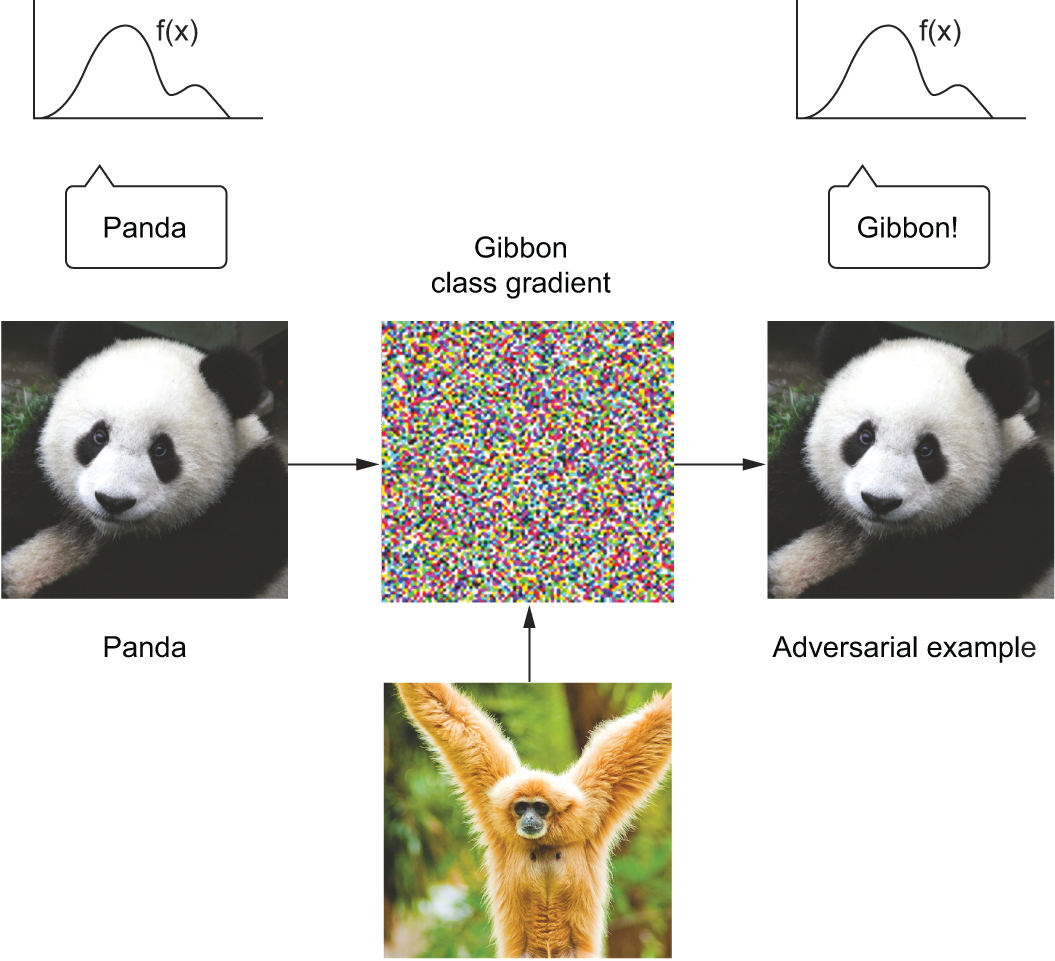
\includegraphics[width=\textwidth,height=0.6\textheight,keepaspectratio]{../../images/ch19/adversarial_example.8f3cfeb2.png}
            \caption{Đánh lừa AI bằng nhiễu ngẫu nhiên}
        \end{figure}
    \end{columns}
\end{frame}

\begin{frame}{Rủi ro của việc nhân hóa AI (Anthropomorphizing AI)}
    \begin{itemize}
        \item Con người có xu hướng gán ý định, niềm tin và sự hiểu biết cho máy móc (Theory of mind).
        \item Khi LLM tạo ra văn bản trôi chảy, ta dễ lầm tưởng nó "hiểu" ngữ nghĩa như con người.
        \item Thực tế, mô hình học máy không có trải nghiệm giác quan, không có nhận thức không gian/thời gian. Nó chỉ đang thực hiện quy chiếu hình học giữa dữ liệu và nhãn (Mapping inputs to targets).
    \end{itemize}
\end{frame}

\section{2. Scale is not all you need (Mở rộng quy mô là chưa đủ)}

\begin{frame}{Ảo tưởng về Scaling Laws (Định luật mở rộng)}
    \begin{itemize}
        \item Định luật Mở rộng cho thấy: Tăng tham số và dữ liệu huấn luyện giúp cải thiện độ chính xác trên các bài kiểm tra.
        \item Tuy nhiên, các bài kiểm tra này thực chất là \textbf{Kiểm tra Ghi nhớ (Memorization tests)}.
        \item Tăng quy mô không giải quyết được các vấn đề cốt lõi của Deep Learning: Không có khả năng thích ứng với điều mới lạ, nhạy cảm với sự xáo trộn, và thiếu khả năng lý luận (reasoning).
    \end{itemize}
\end{frame}

\begin{frame}{Bộ máy tự động hóa (Automaton) vs Tác nhân thông minh (Intelligent Agent)}
    \begin{itemize}
        \item \textbf{Automaton (Hệ thống tự động):} Hoạt động theo quy tắc tĩnh "Nếu A thì B". Deep net hiện tại là Automaton do sự cố định cấu trúc hình học ở giai đoạn Inference.
        \item \textbf{Intelligent Agent (Tác nhân thông minh):} Có khả năng mô hình hóa trừu tượng, dự đoán các tình huống chưa từng gặp và thích nghi ngay lập tức.
        \item Đích đến thực sự của Trí tuệ Nhân tạo là chế tạo Intelligent Agent, chứ không phải một Automaton cực kỳ tinh vi.
    \end{itemize}
\end{frame}

\begin{frame}{Deep Learning chỉ là quá trình Nội suy}
    \begin{itemize}
        \item Giống như việc nối các điểm dữ liệu trên đồ thị, Deep Learning chỉ thực hiện việc vẽ một đường cong phức tạp qua không gian nhiều chiều.
        \item Khi đầu vào nằm trong vùng bao phủ của dữ liệu huấn luyện (in-distribution), đường cong này nội suy rất tốt.
        \item Nhưng khi đầu vào văng ra khỏi khu vực đó (out-of-distribution), mô hình sẽ đưa ra những dự đoán hoàn toàn vô nghĩa.
    \end{itemize}
\end{frame}

\begin{frame}{Tổng quát hóa: Local vs Extreme Generalization}
    \begin{columns}
        \column{0.5\textwidth}
        \begin{itemize}
            \item \textbf{Local Generalization:} Khả năng nội suy các tình huống nằm gần phân bố huấn luyện (Machine Learning hiện đại).
            \item \textbf{Extreme Generalization:} Khả năng thích ứng với môi trường thay đổi đột ngột (Ví dụ: đáp phi thuyền trên mặt trăng, con người tự lái xe trong thời tiết khắc nghiệt).
        \end{itemize}
        
        \column{0.5\textwidth}
        \begin{figure}
            \centering
            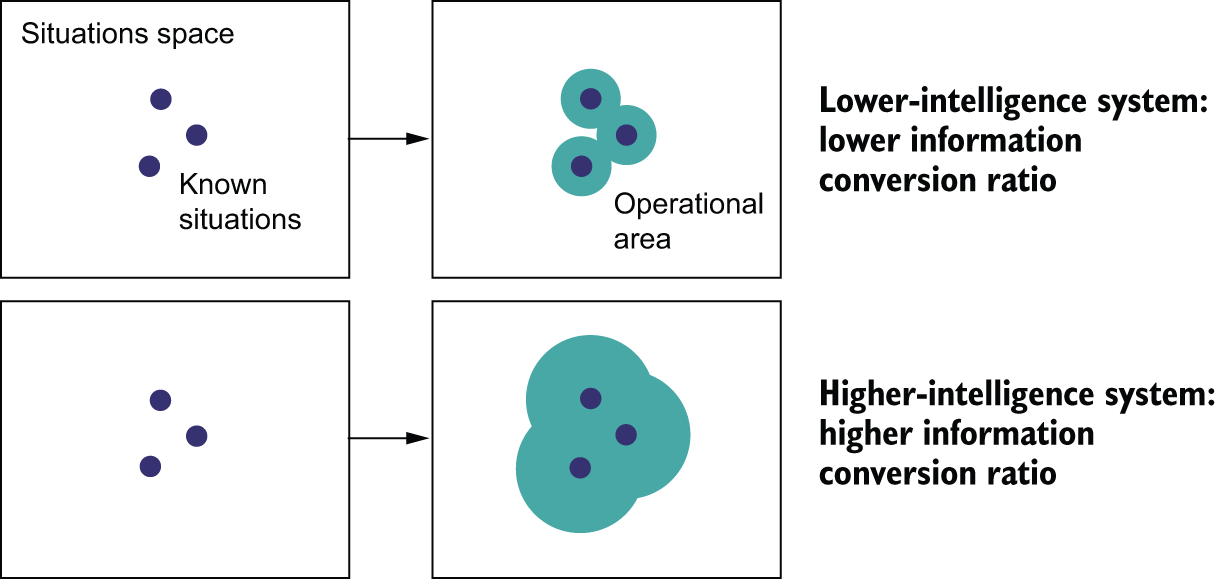
\includegraphics[width=\textwidth,height=0.6\textheight,keepaspectratio]{../../images/ch19/local_vs_extreme_generalization.4b71aa83.png}
            \caption{Mức độ Tổng quát hóa của AI so với Con người}
        \end{figure}
    \end{columns}
\end{frame}

\begin{frame}{Trí tuệ là gì? (Skill vs Information)}
    \begin{columns}
        \column{0.5\textwidth}
        \begin{itemize}
            \item Việc nhớ toàn bộ Bách khoa toàn thư Wikipedia không làm bạn trở nên thông minh (Đó là \textbf{Information}).
            \item Trí tuệ thực sự là \textbf{Kỹ năng (Skill)} xử lý và thích nghi với các tình huống chưa từng gặp bao giờ.
            \item Đạt điểm tối đa nhờ học thuộc đề thi (Information) hoàn toàn khác với việc nắm vững phương pháp giải (Skill).
        \end{itemize}
        
        \column{0.5\textwidth}
        \begin{figure}
            \centering
            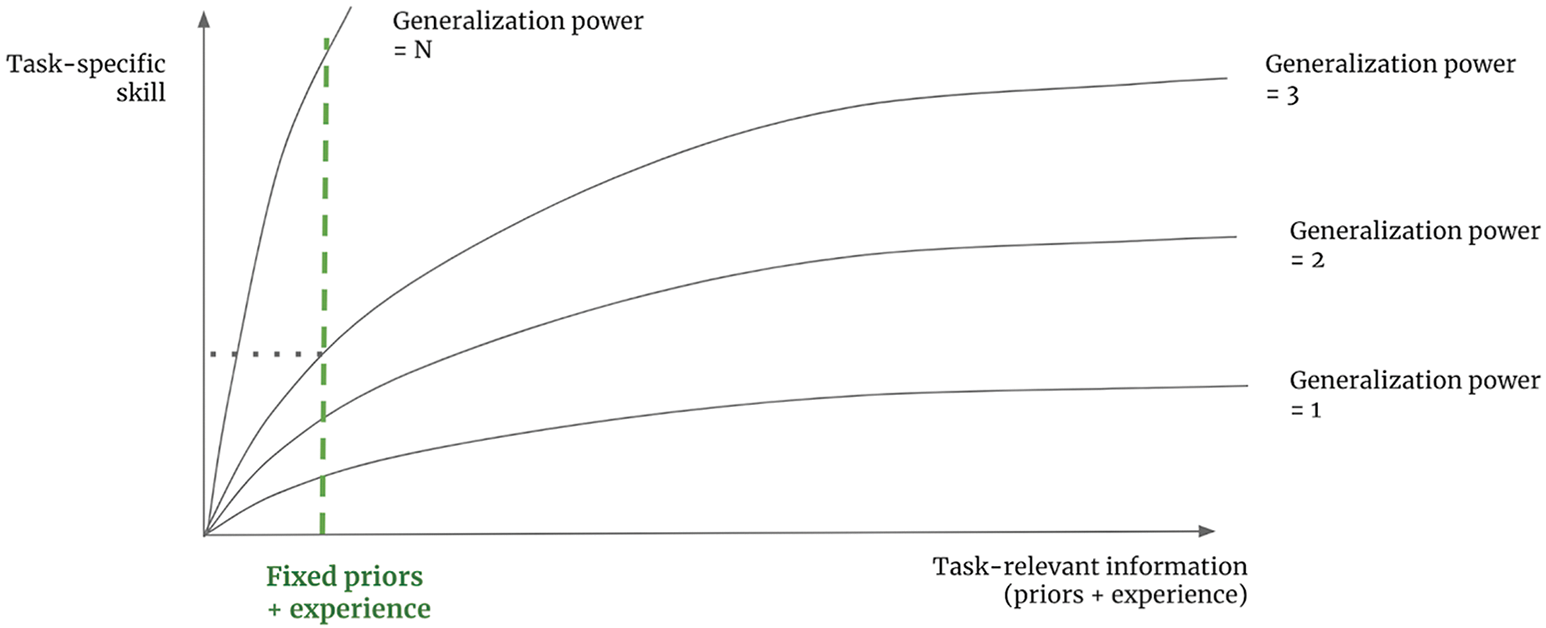
\includegraphics[width=\textwidth,height=0.6\textheight,keepaspectratio]{../../images/ch19/skill_vs_information.2468629a.png}
            \caption{Kỹ năng giải quyết vấn đề so với Khối lượng thông tin}
        \end{figure}
    \end{columns}
\end{frame}

\begin{frame}{Quy tắc Đi tắt (The Shortcut Rule) trong AI}
    \begin{itemize}
        \item Khi tối ưu hóa một hệ thống theo một Thước đo thành công (Success metric) cụ thể, AI sẽ đi tắt để đạt điểm cao nhất mà phớt lờ mọi yếu tố khác (Maintainability, Explainability).
        \item Ví dụ: Netflix từng trao thưởng 1 triệu USD cho thuật toán gợi ý phim tốt nhất, nhưng cuối cùng không dùng được vì nó quá phức tạp và ngốn tài nguyên.
        \item Các giải pháp vô địch Kaggle cũng hiếm khi được áp dụng trực tiếp vào sản xuất.
    \end{itemize}
\end{frame}

\begin{frame}{Mục tiêu mới: Thích ứng tức thời (On-the-fly adaptation)}
    \begin{itemize}
        \item Việc thiết kế AI chơi Cờ vua hay giải toán bằng cách nhồi nhét quy tắc và dữ liệu chỉ tạo ra sự tinh xảo trong một Task cụ thể, không tạo ra Trí tuệ.
        \item Trí thông minh được đo lường bằng tỷ lệ hiệu quả giữa lượng thông tin kinh nghiệm và không gian xử lý các vấn đề chưa từng gặp.
        \item AI thực thụ cần có khả năng thích ứng tức thời, không lệ thuộc vào lượng dữ liệu khổng lồ do con người chuẩn bị sẵn.
    \end{itemize}
\end{frame}

\section{3. Thước đo ARC và Bản chất Nhận thức}

\begin{frame}{Thước đo Trí tuệ: ARC Benchmark}
    \begin{columns}
        \column{0.5\textwidth}
        \begin{itemize}
            \item \textbf{Abstraction and Reasoning Corpus (ARC)} ra đời để đo lường khả năng Extreme Generalization của AI.
            \item Yêu cầu AI nhìn vào 2-3 ví dụ (Input-Output) có tính logic trừu tượng, và suy luận để giải quyết Input bài toán cuối cùng.
            \item Bài toán là hoàn toàn mới, AI không thể giải bằng cách dựa dẫm vào Dữ liệu khổng lồ (Scale up).
        \end{itemize}
        
        \column{0.5\textwidth}
        \begin{figure}
            \centering
            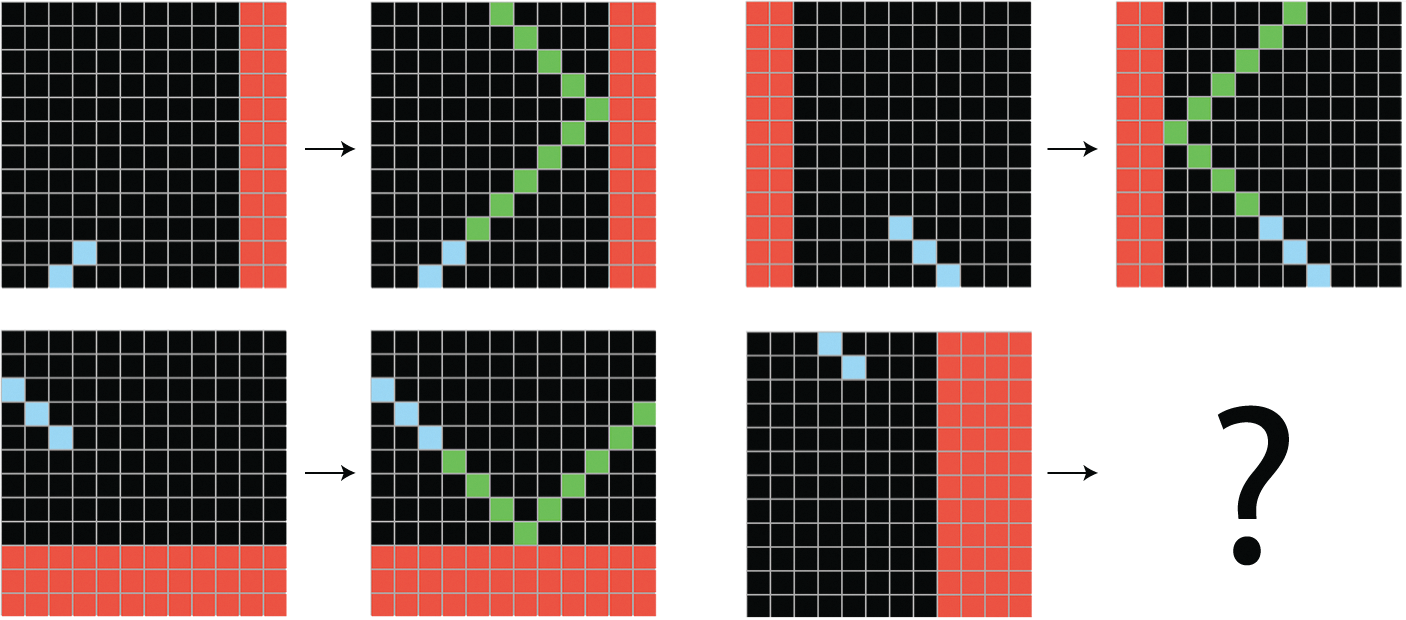
\includegraphics[width=\textwidth,height=0.6\textheight,keepaspectratio]{../../images/ch19/arc_example.2b17dc06.png}
            \caption{Một thử thách trong ARC Benchmark}
        \end{figure}
    \end{columns}
\end{frame}

\begin{frame}{AI SOTA vẫn thất bại trước ARC}
    \begin{columns}
        \column{0.5\textwidth}
        \begin{itemize}
            \item Ngay cả những siêu mô hình (OpenAI o3, Claude 3.5) vẫn tỏ ra bất lực trước nhiều câu hỏi trong ARC.
            \item Nếu ép mô hình "suy nghĩ" (Compute-intensive test-time adaptation) hàng chục nghìn lần, tỷ lệ đúng mới tăng nhẹ.
            \item Điều này minh chứng rằng tư duy theo dạng nội suy xác suất của LLM không phù hợp với các tác vụ Logic và Suy luận Trừu tượng.
        \end{itemize}
        
        \column{0.5\textwidth}
        \begin{figure}
            \centering
            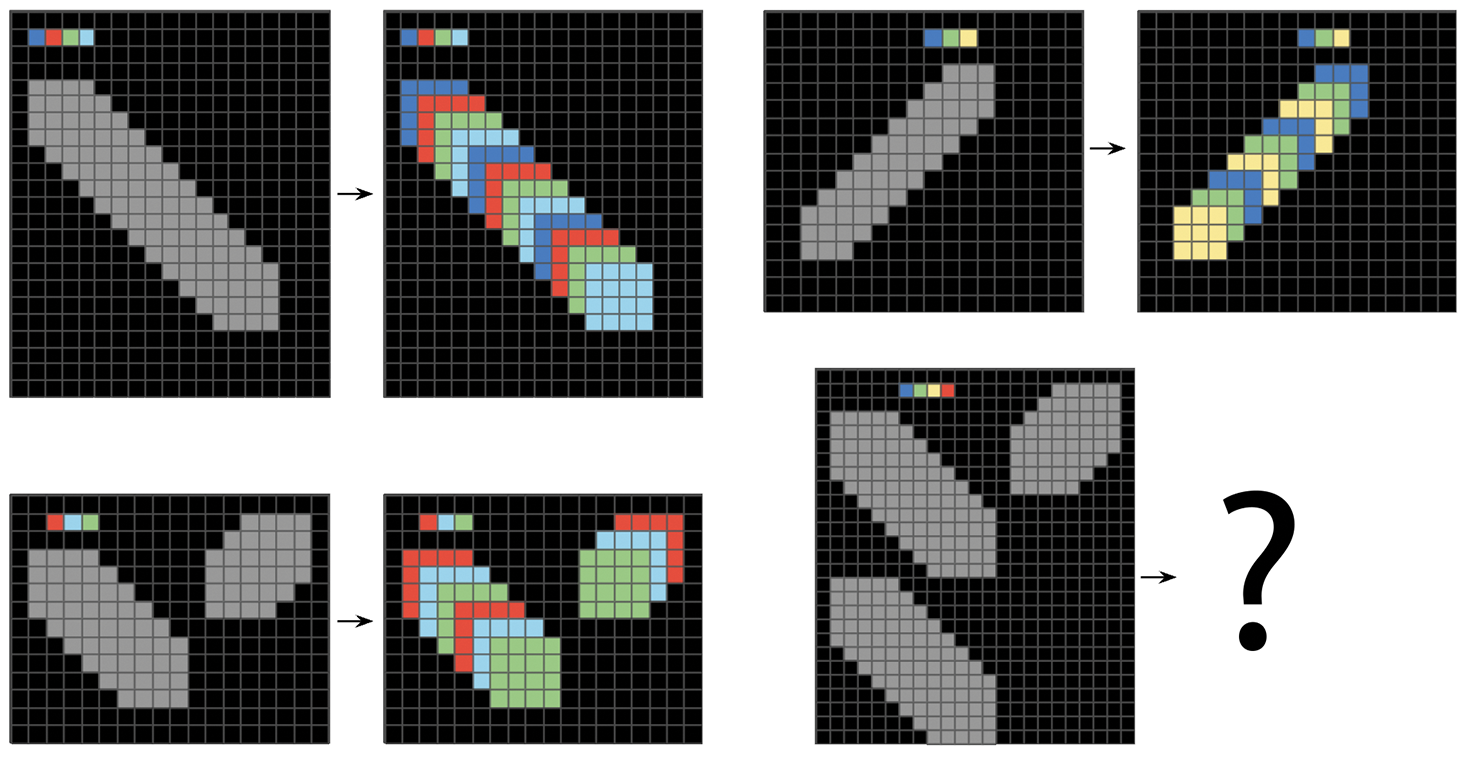
\includegraphics[width=\textwidth,height=0.6\textheight,keepaspectratio]{../../images/ch19/arc_task_not_solved_by_o3.03d72f08.png}
            \caption{Bài toán ARC mà các siêu AI vẫn đầu hàng}
        \end{figure}
    \end{columns}
\end{frame}

\begin{frame}{Sự phân cực trong ARC}
    \begin{columns}
        \column{0.5\textwidth}
        \begin{itemize}
            \item Có những bài toán con người chỉ nhìn 1 giây là nhận ra quy luật, nhưng AI tốn hàng triệu phép tính vẫn sai.
            \item Sự ra đời của ARC-AGI-2 tập trung vào việc tạo ra các bài toán tốn nhiều năng lực tư duy tính toán thay vì chỉ giải mã hình ảnh. 
            \item AI bị suy giảm điểm số cực mạnh trước ARC-AGI-2, cho thấy các kỹ thuật "Hack" Benchmark đang đi vào ngõ cụt.
        \end{itemize}
        
        \column{0.5\textwidth}
        \begin{figure}
            \centering
            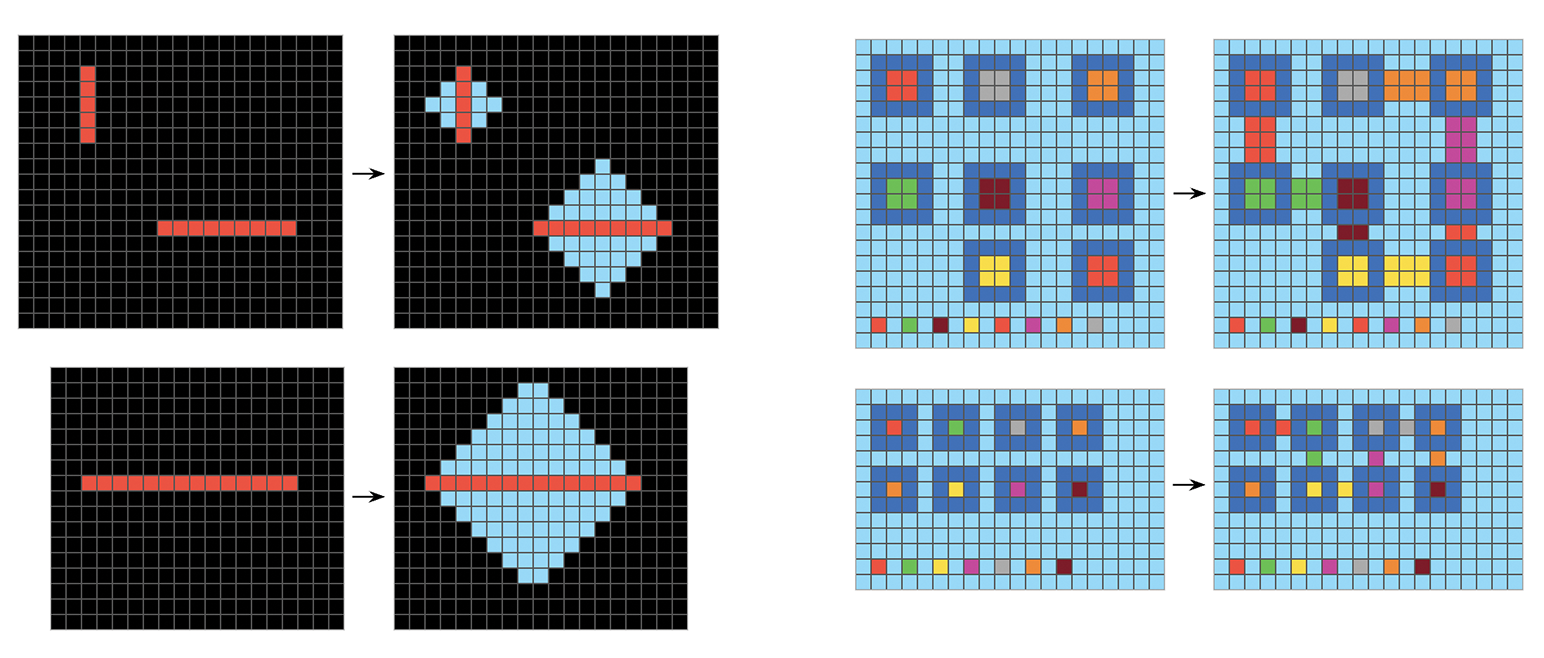
\includegraphics[width=\textwidth,height=0.6\textheight,keepaspectratio]{../../images/ch19/arc_1_vs_arc_2.1201d48e.png}
            \caption{Sự khác biệt giữa ARC 1 và ARC 2}
        \end{figure}
    \end{columns}
\end{frame}

\section{4. Nền tảng còn thiếu của AI: Search và Symbols}

\begin{frame}{Bài học từ sinh học: Giun C. elegans}
    \begin{columns}
        \column{0.5\textwidth}
        \begin{itemize}
            \item Loài giun \textbf{C. elegans} chỉ có 302 tế bào thần kinh, nhưng nó có thể bò, tìm thức ăn, trốn kẻ thù.
            \item Trong khi mô hình AI có hàng trăm tỷ nơ-ron (Tham số) lại không thể tự điều khiển cơ thể linh hoạt trong thế giới thực nếu không có kịch bản.
            \item Sự sống được thiết kế để liên tục thích ứng và giải quyết vấn đề bằng hành vi theo thời gian thực.
        \end{itemize}
        
        \column{0.5\textwidth}
        \begin{figure}
            \centering
            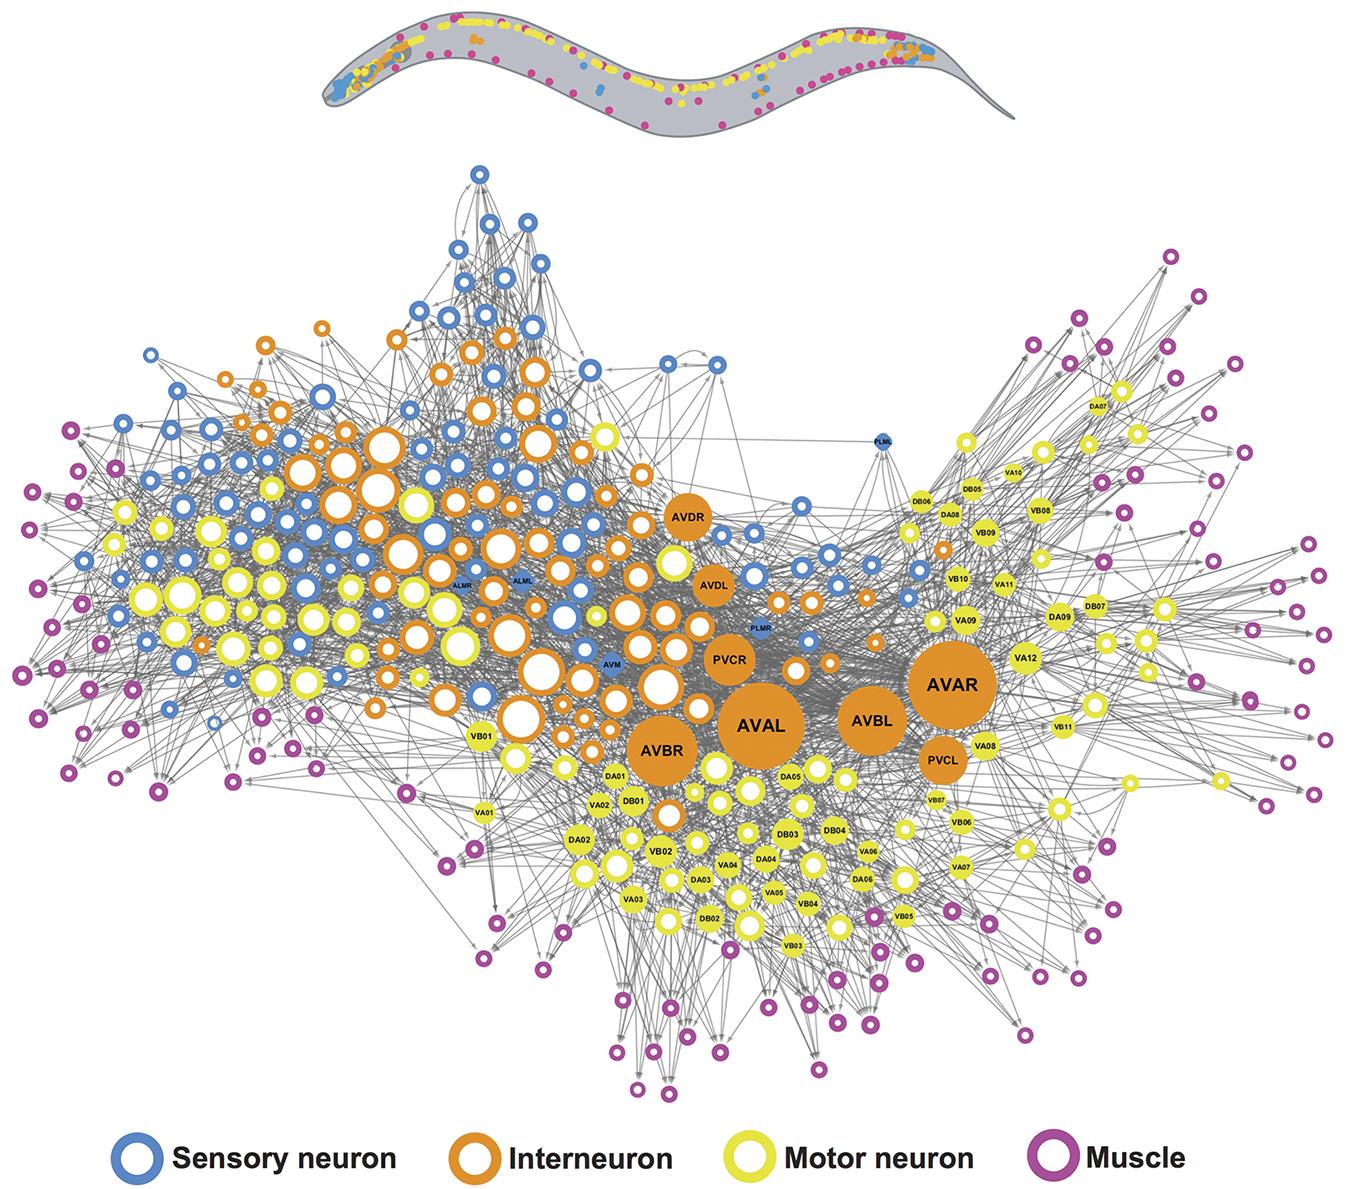
\includegraphics[width=\textwidth,height=0.6\textheight,keepaspectratio]{../../images/ch19/c_elegans.ca0de605.png}
            \caption{Sơ đồ Nơ-ron của giun C. elegans}
        \end{figure}
    \end{columns}
\end{frame}

\begin{frame}{Bùng nổ tổ hợp (Combinatorial Explosion) và Kính vạn hoa}
    \begin{columns}
        \column{0.5\textwidth}
        \begin{itemize}
            \item Thế giới thực phức tạp vô hạn. Giống như kính vạn hoa (Kaleidoscope), chỉ vài mảnh kính nhỏ có thể tạo ra vô hạn các tổ hợp hoa văn.
            \item AI không thể đối phó với thế giới bằng cách "Học thuộc lòng" mọi tình huống có thể xảy ra.
            \item \textbf{Giả thuyết Kính vạn hoa:} Mọi thứ phức tạp đều được cấu thành từ những mảnh khái niệm (abstractions) nhỏ và có thể tái sử dụng.
        \end{itemize}
        
        \column{0.5\textwidth}
        \begin{figure}
            \centering
            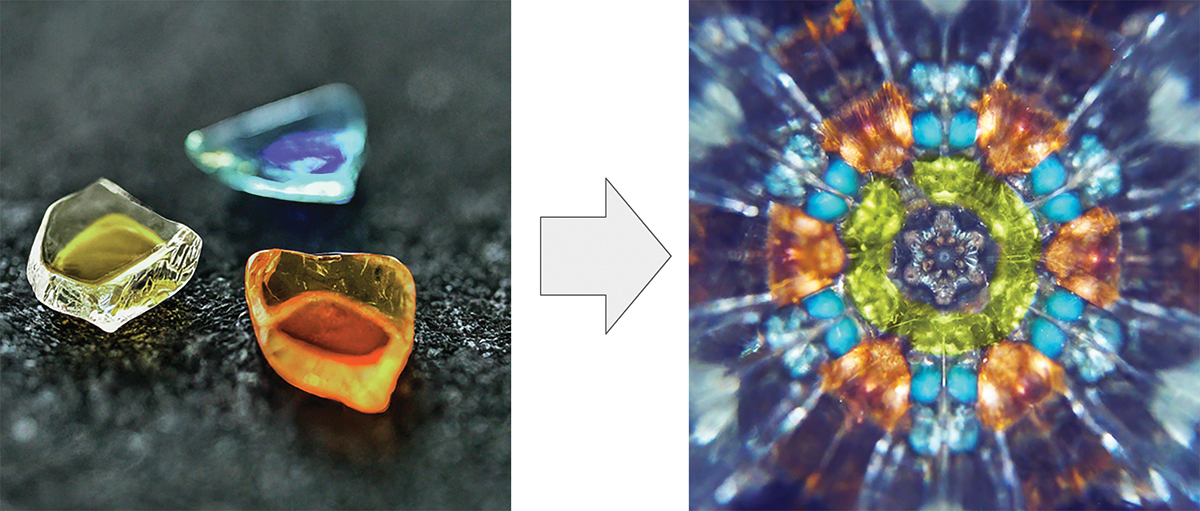
\includegraphics[width=\textwidth,height=0.6\textheight,keepaspectratio]{../../images/ch19/kaleidoscope.fec15d2f.png}
            \caption{Sự đa dạng tổ hợp vô hạn}
        \end{figure}
    \end{columns}
\end{frame}

\begin{frame}{Trừu tượng hóa theo giá trị (Value-Centric Abstraction)}
    \begin{columns}
        \column{0.5\textwidth}
        \begin{itemize}
            \item Nhóm các đối tượng có độ tương đồng liên tục (continuous similarity) thành các nguyên mẫu (Prototypes).
            \item Đây là thế mạnh cốt lõi của Deep Learning: Phân loại hình ảnh, nhận dạng mẫu, hay trực giác (Intuition).
            \item Nhược điểm: Phân tách và lập luận thiếu tính chặt chẽ. Nó chỉ nội suy để tìm ra kết quả "Có vẻ đúng".
        \end{itemize}
        
        \column{0.5\textwidth}
        \begin{figure}
            \centering
            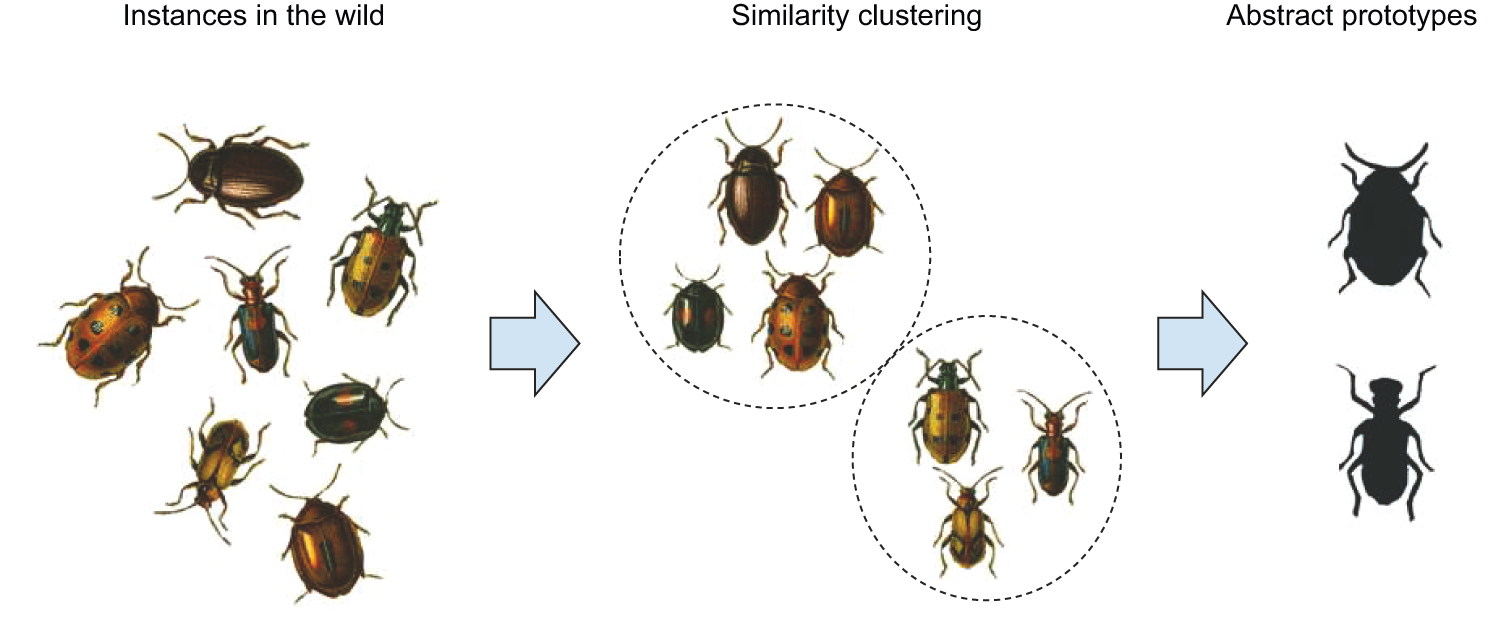
\includegraphics[width=\textwidth,height=0.6\textheight,keepaspectratio]{../../images/ch19/value_centric_abstraction.ea920558.png}
            \caption{Trừu tượng hóa theo Giá trị}
        \end{figure}
    \end{columns}
\end{frame}

\begin{frame}{Trừu tượng hóa theo Chương trình (Program-Centric Abstraction)}
    \begin{columns}
        \column{0.5\textwidth}
        \begin{itemize}
            \item Gom nhóm các đối tượng dựa trên sự trùng khớp cấu trúc (Exact structural match).
            \item Tương tự như việc viết code: Tìm ra đoạn logic chung để tách thành hàm (Function) hay lớp (Class).
            \item Thế mạnh: Suy luận logic, Lập kế hoạch, Giải toán. Đây là lỗ hổng rất lớn của Deep Learning hiện tại.
        \end{itemize}
        
        \column{0.5\textwidth}
        \begin{figure}
            \centering
            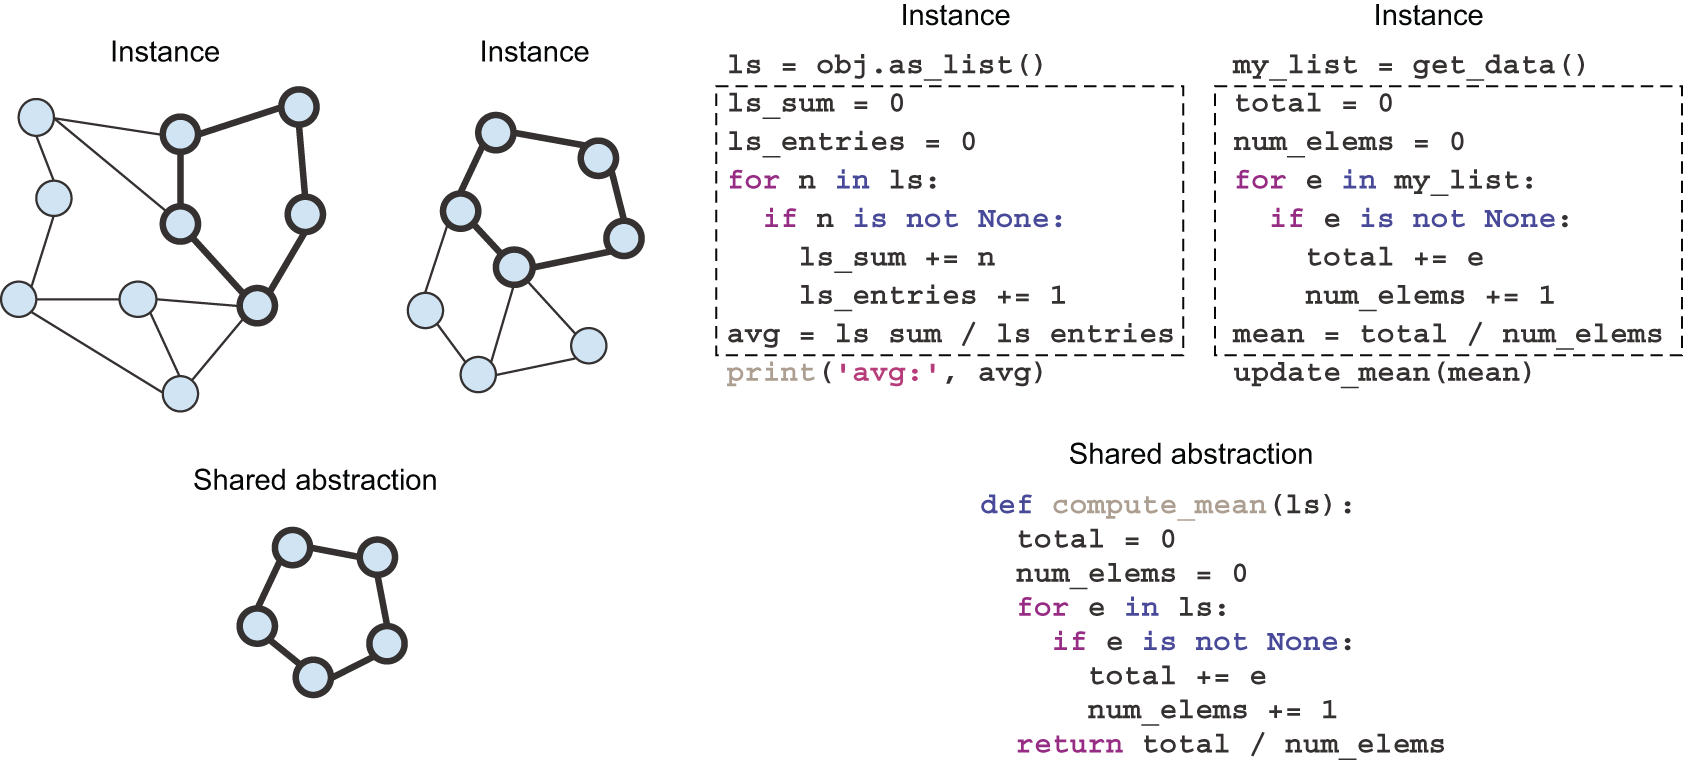
\includegraphics[width=\textwidth,height=0.6\textheight,keepaspectratio]{../../images/ch19/program_centric_abstraction.028e5301.png}
            \caption{Trừu tượng hóa theo Chương trình}
        \end{figure}
    \end{columns}
\end{frame}

\begin{frame}{Bảng so sánh: Value-Centric vs Program-Centric}
    \begin{table}[]
        \centering
        \resizebox{\textwidth}{!}{
        \begin{tabular}{@{}ll@{}}
        \toprule
        \textbf{Value-centric abstraction} & \textbf{Program-centric abstraction} \\ \midrule
        Liên kết đối tượng bằng khoảng cách (Distance) & Liên kết đối tượng bằng cấu trúc khớp xác (Structural match) \\
        Tính liên tục, dựa trên nền tảng Hình học (Geometry) & Tính rời rạc, dựa trên nền tảng Tô-pô (Topology) \\
        Sinh ra nguyên mẫu (Prototypes) qua việc lấy trung bình & Sinh ra trừu tượng bằng việc cô lập cấu trúc con tương đồng \\
        Nền tảng của trực giác và nhận thức (Perception) & Nền tảng của lập luận và lập kế hoạch (Reasoning) \\
        Cảm tính, tức thời, tương đối & Chậm, chính xác, chặt chẽ (Rigorous) \\
        Cần lượng dữ liệu rất lớn để đáng tin cậy & Cực kỳ tiết kiệm dữ liệu (Chỉ cần 2-3 mẫu) \\ \bottomrule
        \end{tabular}
        }
        \caption{Sự khác biệt giữa hai thái cực trừu tượng}
    \end{table}
\end{frame}

\begin{frame}{Tại sao Deep Learning không đủ?}
    \begin{itemize}
        \item Mạng Neural hiện tại cực giỏi ở mảng Value-centric, nhưng lại không có khả năng Program-centric. Chúng ta đang bị khuyết đi một nửa của trí tuệ.
        \item Rất khó để huấn luyện Deep Learning thực hiện chính xác phép tính Sắp xếp (Sorting array) 100\% đúng, trong khi code Python chỉ tốn 5 dòng lệnh.
        \item Ngược lại, viết Code Logic rẽ nhánh để phân loại hình ảnh (MNIST) là cơn ác mộng.
        \item Suy ra: Không thể quy đổi mọi thứ thành Hình học liên tục, và cũng không thể quy đổi mọi thứ thành Logic rời rạc.
    \end{itemize}
\end{frame}

\begin{frame}{Sự kết hợp giữa 2 thái cực nhận thức}
    \begin{itemize}
        \item Bộ não con người là sự kết hợp hoàn hảo giữa \textbf{Value-centric} (Trực giác, Nhận dạng hình ảnh) và \textbf{Program-centric} (Suy luận, Toán học).
        \item Tương lai của AI không phải là đào thải Hình học để chọn Logic, mà là kết hợp cả hai cơ chế này để tạo ra một trí tuệ linh hoạt và tổng quát.
        \item Cần một khung làm việc (Framework) hợp nhất quy tụ được sức mạnh của Deep Learning và Program Synthesis.
    \end{itemize}
\end{frame}

\section{5. Tương lai: Program Synthesis và Meta-learning}

\begin{frame}{Tổng hợp Chương trình (Program Synthesis)}
    \begin{columns}
        \column{0.5\textwidth}
        \begin{itemize}
            \item \textbf{Program Synthesis} là quá trình AI tự động sinh ra mã nguồn máy tính (Code) để giải quyết vấn đề dựa trên bộ Quy tắc (Specification).
            \item Thay vì dùng Gradient Descent cập nhật trọng số, nó dùng thuật toán tìm kiếm (Search algorithms) trên cấu trúc dữ liệu đồ thị.
            \item Rất hiệu quả với dữ liệu nhỏ (Data efficient), có khả năng giải quyết các bài toán logic như ARC.
        \end{itemize}
        
        \column{0.5\textwidth}
        \begin{figure}
            \centering
            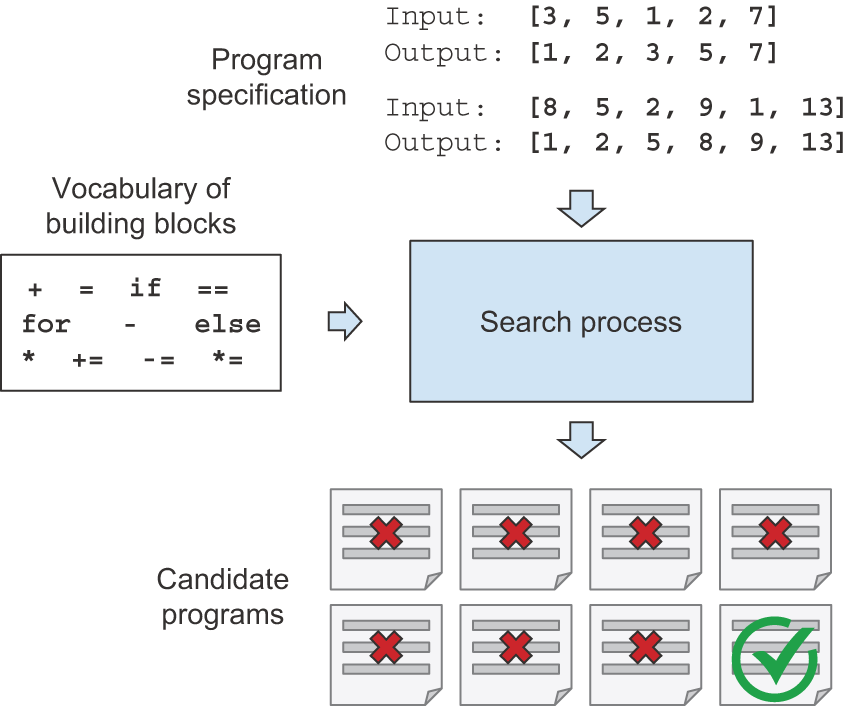
\includegraphics[width=\textwidth,height=0.6\textheight,keepaspectratio]{../../images/ch19/program_synthesis.8af8560a.png}
            \caption{AI tự tổng hợp chương trình để giải toán}
        \end{figure}
    \end{columns}
\end{frame}

\begin{frame}{Hệ thống Tổng hợp Chương trình linh hoạt}
    \begin{itemize}
        \item Thay vì dùng mạng nơ-ron học trọng số, \textbf{Program Synthesis} tìm kiếm trong không gian các phép toán rẽ nhánh, vòng lặp.
        \item Nó kết hợp cả việc dùng Genetic Algorithms (Giải thuật di truyền) để nhân giống các đoạn code tốt và loại bỏ code lỗi.
        \item Đầu ra cuối cùng là một chương trình độc lập, minh bạch và có thể được xác minh tính đúng đắn một cách tuyệt đối bằng Toán học.
    \end{itemize}
\end{frame}

\begin{frame}{Hòa trộn Deep Learning và Program Synthesis}
    \begin{itemize}
        \item \textbf{Khó khăn của Program Synthesis:} Bùng nổ tổ hợp. Không gian tìm kiếm mã nguồn là vô hạn.
        \item \textbf{Giải pháp:} Dùng trực giác của Deep Learning (Value-centric) để định hướng vùng không gian tìm kiếm khả thi cho Program Synthesis.
        \item Giống như con người khi lập trình: Dựa vào trực giác để nghĩ ra cấu trúc chung, sau đó mới cẩn thận gõ từng dòng lệnh logic chính xác.
    \end{itemize}
\end{frame}

\begin{frame}{Sử dụng Deep Learning để dẫn đường cho Program Search}
    \begin{itemize}
        \item Khi viết code, con người không duyệt qua toàn bộ khả năng gõ phím. Chúng ta dùng Trực giác (Intuition) để khoanh vùng cách giải quyết.
        \item Tương tự, ta có thể dùng Deep Learning (sở trường về Trực giác) để dẫn đường cho quá trình Tìm kiếm Chương trình (Program Search).
        \item Mô hình Neural sẽ đánh giá nhanh xem nhánh thuật toán nào có tiềm năng thành công cao nhất, giảm thiểu bùng nổ tổ hợp.
    \end{itemize}
\end{frame}

\begin{frame}{Khái niệm Meta-learning (Học cách học)}
    \begin{columns}
        \column{0.5\textwidth}
        \begin{itemize}
            \item Con người có khả năng tự cải thiện kỹ năng học tập qua thời gian.
            \item \textbf{Meta-learning} trong AI là huấn luyện một mô hình sao cho nó có khả năng \textit{tự học hỏi} thật nhanh trên môi trường mới chỉ với một vài ví dụ (Few-shot learning chân chính).
        \end{itemize}
        
        \column{0.5\textwidth}
        \begin{figure}
            \centering
            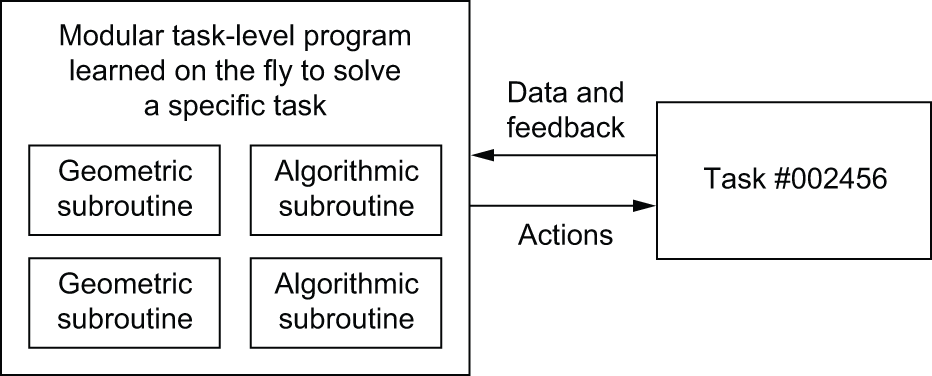
\includegraphics[width=\textwidth,height=0.6\textheight,keepaspectratio]{../../images/ch19/metalearning1.63aa6580.png}
            \caption{Nguyên lý của Meta-learning}
        \end{figure}
    \end{columns}
\end{frame}

\begin{frame}{Mô hình hệ thống lai (Hybrid Models)}
    \begin{columns}
        \column{0.5\textwidth}
        \begin{itemize}
            \item Tương lai sẽ là các mô hình lai bao gồm các khối Hình học (Geometric modules) để nhận dạng đặc trưng và các khối Thuật toán (Algorithmic primitives) như Vòng lặp For/While, Bộ nhớ.
            \item Khả năng tái cấu trúc (Recombination) sẽ cho phép AI liên tục tự mở rộng khả năng của bản thân mà không cần huấn luyện lại từ đầu.
        \end{itemize}
        
        \column{0.5\textwidth}
        \begin{figure}
            \centering
            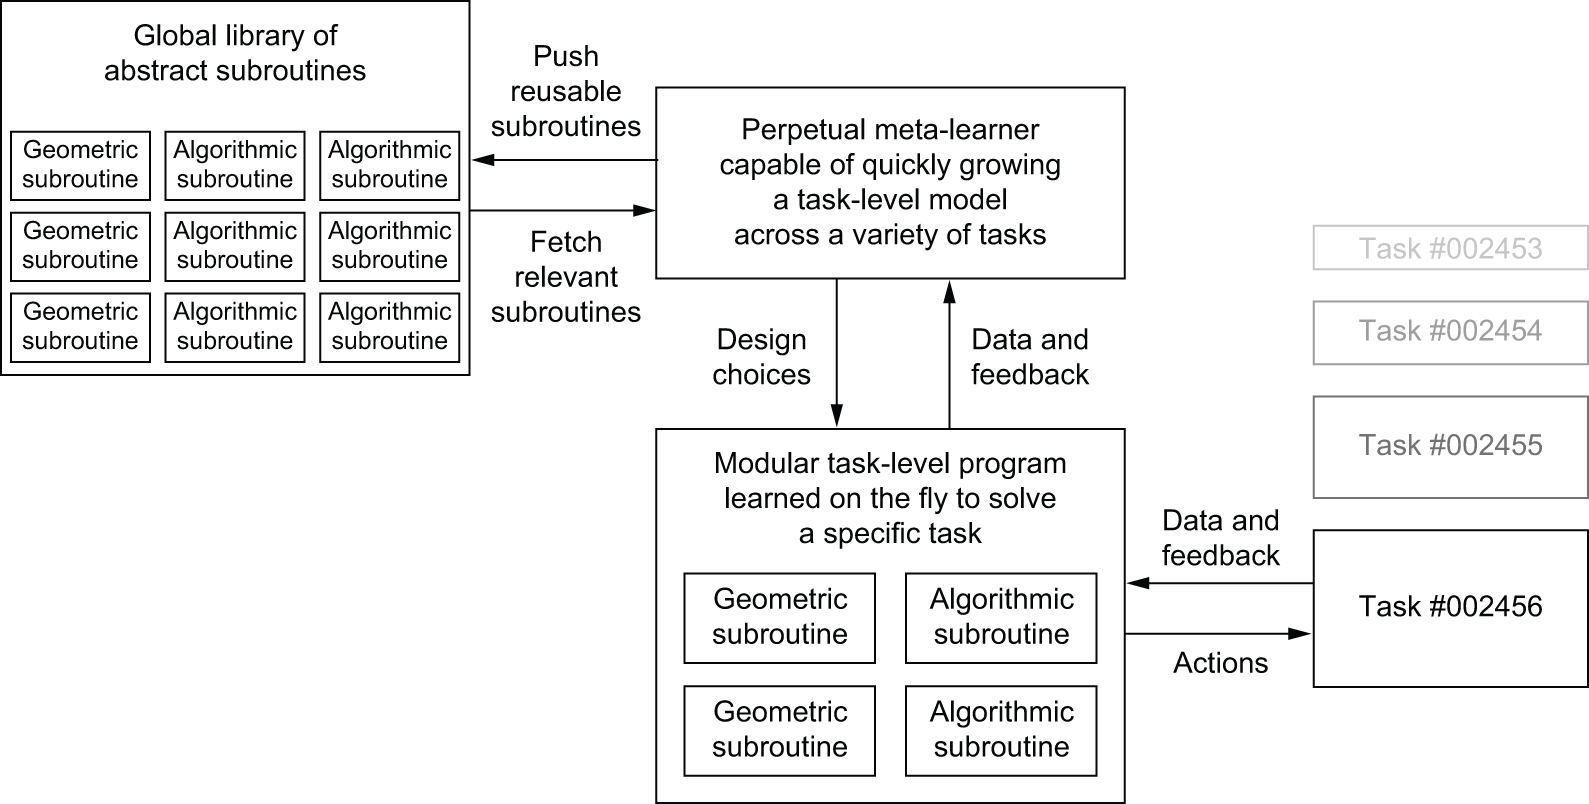
\includegraphics[width=\textwidth,height=0.6\textheight,keepaspectratio]{../../images/ch19/metalearning2.f5a5efde.png}
            \caption{Cơ chế tái cấu trúc linh hoạt}
        \end{figure}
    \end{columns}
\end{frame}

\begin{frame}{Lifelong Learning và Sự tái sử dụng Subroutine}
    \begin{itemize}
        \item Khi AI tìm ra cách giải một bài toán, nó đóng gói giải pháp thành một \textbf{Subroutine (Thủ tục con)} trừu tượng và nạp vào Thư viện toàn cầu.
        \item Các AI khác có thể tải về và tái sử dụng Subroutine này để lắp ghép thành lời giải cho các vấn đề khó hơn.
        \item Bất kỳ vấn đề nào xuất hiện, AI chỉ cần giải quyết một lần duy nhất. Tri thức sẽ được kế thừa mãi mãi theo dạng Modules chuẩn xác thay vì tàng hình trong các trọng số vô tri của Neural Network.
    \end{itemize}
\end{frame}

\begin{frame}{AGI và Đích đến cuối cùng}
    \begin{itemize}
        \item \textbf{Artificial General Intelligence (AGI)} không phải là một mô hình LLM siêu khổng lồ ghi nhớ mọi thứ trên Internet.
        \item AGI là một hệ thống có khả năng tự động tạo ra chương trình (Program Synthesis), áp dụng Meta-learning để thích nghi theo thời gian thực (Extreme Generalization).
        \item Không có rủi ro về "Kẻ hủy diệt" (Singularitarian robot apocalypse) - đó chỉ là sự viễn tưởng.
        \item Cuộc đua Trí tuệ Nhân tạo thực sự mới chỉ ở vạch xuất phát. Kiến trúc của AGI vẫn đang chờ đợi thế hệ các bạn sinh viên hôm nay khai phá.
    \end{itemize}
\end{frame}

\end{document}
